\section{Задача 2.3}
\subsection{Задание:}
$
	\begin{cases}
		(1 + i)x + (1 + 2i)y + (1 + 3i)z + (1 + 4i)t = 1 + 5i \\
		(3 - i)x + (4 - 2i)y + (1 + i)z + 4it = 2 - i
	\end{cases}
$
\subsection{Решение:}
Преобразуем систему:
\\[1em]
$
	\begin{cases}
		x + y + z + t = 1 \\
		3x + 4y + z = 2 \\
		ix + 2iy + 3iz + 4it = 5i \\
		-ix -2iy + iz + 4it = -i
	\end{cases}
$
\\[1em]
Разделим последние две строчки на $ i $:
\\[1em]
$
\begin{cases}
	x + y + z + t = 1 \\
	3x + 4y + z = 2 \\
	x + 2y + 3z + 4t = 5 \\
	-x -2y + z + 4t = -1
\end{cases}
$
\\[1em]
Решим систему методом Крамера:
\\[1em]
$
	\Delta =
	\begin{vmatrix}
		1 & 1 & 1 & 1 \\
		3 & 4 & 1 & 0 \\
		1 & 2 & 3 & 4 \\
		-1 & -2 & 1 & 4 \\
	\end{vmatrix} = 8
	\\[1em]
	\Delta_x =
	\begin{vmatrix}
		1 & 1 & 1 & 1 \\
		2 & 4 & 1 & 0 \\
		5 & 2 & 3 & 4 \\
		-1 & -2 & 1 & 4 \\
	\end{vmatrix} = -16
	\\[1em]
	\Delta_y =
	\begin{vmatrix}
		1 & 1 & 1 & 1 \\
		3 & 2 & 1 & 0 \\
		1 & 5 & 3 & 4 \\
		-1 & -1 & 1 & 4 \\
	\end{vmatrix} = 12
	\\[1em]
	\Delta_z =
	\begin{vmatrix}
		1 & 1 & 1 & 1 \\
		3 & 4 & 2 & 0 \\
		1 & 2 & 5 & 4 \\
		-1 & -2 & -1 & 4 \\
	\end{vmatrix} = 16
	\\[1em]
	\Delta_t =
	\begin{vmatrix}
		1 & 1 & 1 & 1 \\
		3 & 4 & 1 & 2 \\
		1 & 2 & 3 & 5 \\
		-1 & -2 & 1 & -1 \\
	\end{vmatrix} = -4
	\\[1em]
	x = \dfrac{\Delta_x}{\Delta} = -2 \\[1em]
	y = \dfrac{\Delta_y}{\Delta} = \dfrac{3}{2} \\[1em]
	z = \dfrac{\Delta_z}{\Delta} = 2 \\[1em]
	t = \dfrac{\Delta_t}{\Delta} = - \dfrac{1}{2} \\[1em]
$
\subsection{Выполним компьютерную проверку в среде Wolfram Mathematica:}
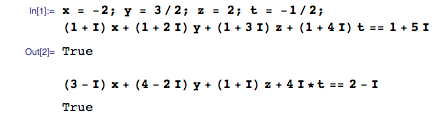
\includegraphics[scale=0.6]{task/2_03/screen1.png}
\subsection{Вывод:}
Мы верно нашли решение системы.
